\chapter{TypeScript + p5.js を始める}
\label{chap:introduction}

この章では、TypeScript + p5.js のプログラムを自分のWindows環境で動かすための準備を行います。まだTypeScriptの詳しい文法やp5.jsの仕組みは深く説明しません。まずは、教材を取得し、プログラムを実行し、少し書き換え、Gitで保存するところまでを体験します。

\section{この章で行うこと}

プログラミングを学ぶときには、プログラムを書くためのエディタ、教材を取得するためのGit、プログラムを動かすためのNode.jsが必要になります。この章では、それらを順番に準備します。

\begin{itemize}
    \item VS Codeをインストールする
    \item Node.jsをインストールする
    \item Gitをインストールする
    \item 教材をGitHubから取得する
    \item VS Codeで教材フォルダを開く
    \item 必要なライブラリをインストールする
    \item 開発サーバを起動する
    \item プログラムを実行してみる
    \item プログラムを書き換えてみる
    \item Gitで変更を保存する
\end{itemize}

\begin{pointbox}{この章の目標}
この章の目標は、TypeScript + p5.js のプログラムをブラウザで表示できる状態にすることです。文法をすべて理解する必要はありません。まずは「動いた」という状態を作ることを優先します。
\end{pointbox}

\section{JavaScriptとTypeScriptの関係}

この教材で使う言語はTypeScriptです。
TypeScriptはJavaScriptをベースに、「型（データの種類の情報）」を追加した言語です。
TypeScriptは、開発中に書く言語で、実行するときにはJavaScriptに変換されます。
型情報を付けることで、間違った値を渡したときに実行前に気づきやすくなります。
JavaScriptはブラウザやNode.jsでそのまま動く言語で、Web開発では最も広く使われています。
JavaScriptはそのままでも十分強い言語ですが、規模の大きいプログラムでは次のような悩みが出やすくなります。

\begin{itemize}
    \item 関数にどんな値を渡すのかが分かりづらい
    \item 変数の値がいつどう変わるのか追いにくい
    \item チームで分担して開発すると、読み手ごとの解釈差が起きる
\end{itemize}

TypeScriptはこれらに対して、型注釈\footnote{英語ではtype annotationと呼びます。}
を通して「この値は何を表すのか」を明示しやすくします。
実行時にはTypeScriptを一度JavaScriptに変換しますが、書くときは型の手掛かりで理解しやすいコードになります。

近年TypeScriptが広く使われている理由は、JavaScriptの開発現場で「動きはそのままに、変更に強い構造」を求める流れが強まったためです。教材の中でも、変数・関数・クラスなどの概念を型付きで学ぶことで、次の章からのプログラミングがやりやすくなることを目指します。

\section{p5.jsとは何か}

p5.jsは、JavaScriptで図形、色、アニメーション、マウスやキーボードの操作などを扱いやすくするためのライブラリです。
この教材では、TypeScriptでプログラムを書き、p5.jsの機能を使って画面に図形を描いたり、動きのある作品を作ったりします。

p5.jsは、メディアアート系のプログラムを作るための言語であるProcessingの影響を受けて作られました。
Webブラウザで動くJavaScriptライブラリとして、図形を描き、動かし、操作に反応するプログラムを作るための機能を提供します。

p5.jsを利用して作ったプログラムのことを、よく\textbf{スケッチ}と呼びます。
スケッチという言葉には、絵やアイデアを試しながら形にしていくという意味があります。
この教材でも、p5.jsで作るひとまとまりのプログラムをスケッチと呼ぶことがあります。

\begin{pointbox}{p5.jsの背景}
p5.jsは、JavaScriptに図形の描画や入力の機能を加えるライブラリです。プログラムの中でp5.jsを読み込むと、これらの機能を使えます。
\end{pointbox}

\section{Node.jsとは何か}

Node.jsは、ブラウザの外でJavaScriptを動かすための実行環境です。
もともとJavaScriptはWebブラウザの中で動く言語として使われてきました。
しかし、TypeScriptをJavaScriptへ変換したり、開発用のサーバを起動したりする作業では、ブラウザの外でもJavaScriptの仕組みを使う必要があります。
そのために使うのがNode.jsです。

この教材では、Node.jsそのものを詳しく学ぶわけではありません。
Node.jsは、TypeScript + p5.jsの教材プロジェクトを動かすための土台として使います。
たとえば、\texttt{npm install}で必要なライブラリを準備したり、\texttt{npm run dev}でブラウザ確認用の開発サーバを起動したりします。

\begin{pointbox}{Node.jsとnpm}
Node.jsをインストールすると、\texttt{npm}というコマンドも一緒に使えるようになります。
\texttt{npm}は、p5.jsやTypeScriptなど、プロジェクトに必要なライブラリを準備するための道具です。
\end{pointbox}

\section{Gitとは何か}

Gitは、ファイルの変更履歴を記録するための道具です。
プログラムを書いていると、最初はうまく動いていたのに、少し書き換えたあとで動かなくなることがあります。
そのようなとき、Gitで途中の状態を記録しておくと、「どこで何を変更したのか」をあとから確認できます。

Gitは、単にファイルを保存する道具ではありません。
VS Codeでファイルを保存すると、現在の内容が上書きされます。
一方、Gitでは「この時点の変更を記録する」という形で、作業の節目を残します。
この記録を\textbf{コミット}と呼びます。

\begin{pointbox}{Gitでできること}
Gitを使うと、変更したファイルの一覧を確認したり、作業の節目を記録したりできます。
また、GitHubのようなサービスと組み合わせると、教材ファイルの配布や、複数のPCでの作業もしやすくなります。
\end{pointbox}

最初のうちは、Gitの仕組みをすべて理解する必要はありません。
この章では、次の3つの流れを覚えれば十分です。
\texttt{git status}で状態を確認し、\texttt{git add}で保存対象を選び、\texttt{git commit}で変更の記録を作ります。

Gitの考え方は少し抽象的なので、動画で全体像を見ておくのも役に立ちます。
次の動画は、Gitの導入として比較的見やすい内容です。
\url{https://www.youtube.com/watch?v=6SLMB7BPG9E}

もう少し詳しい説明として、次の動画も参考になります。
学生にとって少し難しく感じるかもしれませんが、Gitが何を解決する道具なのかを知る助けになります。
\url{https://www.youtube.com/watch?v=WMIiPcgGC4Q}

\section{VS Codeをインストールする}

VS Codeは、プログラムを書くためのエディタです。TypeScriptのプログラムを読みやすく表示したり、間違いを見つけやすくしたりする機能があります。

WebブラウザでVisual Studio Codeの公式サイトを開き、Windows用のインストーラをダウンロードします。インストーラを起動したら、画面の指示に従ってインストールしてください。

\begin{notebox}{インストール時の注意}
インストール中に「PATHに追加する」や「Codeで開く」という項目が表示された場合は、有効にしておくと便利です。授業中に設定が異なっていても大きな問題にはなりませんが、フォルダを右クリックしてVS Codeで開けるようになります。
\end{notebox}

\section{Node.jsをインストールする}

Node.jsは、TypeScriptやp5.jsを使った教材プロジェクトを動かすために必要な実行環境です。Node.jsをインストールすると、\texttt{npm}というコマンドも一緒に使えるようになります。

WebブラウザでNode.jsの公式サイトを開き、LTSのWindows Installer（\texttt{.msi}）をダウンロードします。LTS版は、長く安定して使うための版です。教材で使うVite 8は、Node.js 20系では20.19.0以上、22系では22.12.0以上が必要です。Node.js公式サイトの現在のLTS版インストーラはこの条件を満たします。すでに古いNode.jsがインストールされている場合は、LTS版に更新してから使ってください。インストーラでは標準設定のまま進め、インストールを最後まで完了してください。

インストールが終わったら、開いているVS CodeとPowerShellをいったん閉じてから、もう一度開きます。新しく開いたターミナルで、次のコマンドを一行ずつ実行し、Node.jsとnpmが使えるか確認します。

\begin{listing}[htbp]
\begin{minted}{powershell}
node -v
npm -v
\end{minted}
\caption{Node.jsとnpmのバージョン確認}
\label{lst:chapter01-check-node}
\end{listing}

Node.jsでは\texttt{v}で始まる値、npmでは数字で始まるバージョン番号が表示されれば、Node.jsとnpmを使う準備ができています。なお、すでに古いNode.jsが入っている場合は、Vite 8の条件を満たすために更新が必要になることがあります。

\begin{notebox}{コマンドが認識されないとき}
\texttt{node}や\texttt{npm}が「コマンドとして認識されません」と表示されたときは、まずターミナルを閉じて開き直します。それでも直らないときはWindowsを再起動してください。再起動後も実行できない場合は、表示されたメッセージを添えて担当者に相談してください。
\end{notebox}

\section{Gitをインストールする}

Gitは、プログラムの変更を記録するための道具です。この教材では、GitHubに置かれている教材ファイルを取得するときにもGitを使います。

WebブラウザでGit for Windowsの公式サイトを開き、Windows用のインストーラをダウンロードします。インストール項目はたくさんありますが、最初は基本的に標準設定のままで構いません。

インストールが終わったら、VS Codeのターミナルで次のコマンドを実行して、Gitが使えることを確認します。この章では、コマンドをPowerShellで実行する手順に統一します。

\begin{listing}[htbp]
\begin{minted}{powershell}
git --version
\end{minted}
\caption{Gitのバージョンを確認するコマンド}
\label{lst:chapter01-check-git}
\end{listing}

続いて、Gitに記録する名前とメールアドレスを設定します。次の\texttt{Taro Student}と\texttt{taro@example.com}は自分の情報に置き換えてください。メールアドレスには、授業の作業に使うことを許可されているものを指定します。

\begin{listing}[htbp]
\begin{minted}{powershell}
git config --global user.name "Taro Student"
git config --global user.email "taro@example.com"
\end{minted}
\caption{Gitに名前とメールアドレスを設定するコマンド}
\label{lst:chapter01-git-identity}
\end{listing}

\section{教材をGitHubから取得する}

教材のファイルはGitHubから取得します。GitHubは、プログラムや教材ファイルを保存・共有するためのサービスです。

まず、教材を保存したいフォルダを決めます。たとえば、ドキュメントフォルダの中に授業用のフォルダを作っておくと管理しやすくなります。PowerShellでは、次のように現在のフォルダを移動してから\texttt{git clone}を実行します。

\begin{listing}[htbp]
\begin{minted}{powershell}
Set-Location ([Environment]::GetFolderPath("MyDocuments"))
Get-Location
mkdir work-textbook
cd work-textbook
git clone https://github.com/m-riho/typescript-p5js-programming-textbook.git
\end{minted}
\caption{教材を保存するフォルダを作成してリポジトリを取得するコマンド}
\label{lst:chapter01-git-clone}
\end{listing}

\texttt{Set-Location}は、Windowsに登録されているドキュメントフォルダへ移動します。ドキュメントフォルダの名前や保存場所がPCごとに異なっても、\texttt{GetFolderPath("MyDocuments")}が実際の場所を調べます。続く\texttt{Get-Location}には現在いる場所が表示されるので、エクスプローラーのドキュメントフォルダと同じ場所か確認してください。

上のURLは、この教材の学生向け公開リポジトリの正式なURLです。\texttt{git clone}は通常、最初に教材を取得するときに一度だけ実行します。実行が終わると、\texttt{work-textbook}の中に\texttt{typescript-p5js-programming-textbook}フォルダが作られます。

\begin{notebox}{フォルダ名に注意する}
Windowsでは、フォルダ名に日本語や空白が含まれていても多くの場合は動作します。ただし、コマンド入力に慣れるまでは、\texttt{work-textbook}のような英数字だけのフォルダ名にしておくとトラブルを減らせます。
\end{notebox}

\section{VS Codeで教材フォルダを開く}

教材を取得したら、VS Codeでそのリポジトリのルートフォルダを開きます。VS Codeのメニューから「ファイル」→「フォルダーを開く」を選び、\texttt{git clone}で作られた教材フォルダを指定します。

フォルダを開いたら、VS Codeの画面左側にあるエクスプローラーで\texttt{chapters/}、\texttt{listings/}、\texttt{typescript-p5/}が表示されることを確認します。プログラムを書くときは、このフォルダを開いた状態で作業します。

初めて開くフォルダでは、ワークスペースを信頼するか尋ねる画面が表示されることがあります。授業で配布されたリポジトリを開いていることを確認してから、信頼する選択肢を選びます。統合ターミナルは、VS Codeのメニューから「ターミナル」→「新しいターミナル」を選ぶと開けます。

\section{必要なライブラリをインストールする}

教材プロジェクトには、p5.jsやTypeScriptなど、プログラムを動かすために必要なライブラリが含まれています。ただし、GitHubから取得した直後は、ライブラリ本体はまだ手元に入っていません。

VS Codeで教材リポジトリのルートフォルダを開いた状態で、メニューから「ターミナル」→「新しいターミナル」を選びます。画面下部にターミナルが開いたら、次のコマンドを上から順に実行します。

\begin{listing}[htbp]
\begin{minted}{powershell}
cd typescript-p5
Get-Location
Get-ChildItem package.json
npm install
\end{minted}
\caption{実行用プロジェクトで必要なライブラリをインストールするコマンド}
\label{lst:chapter01-npm-install}
\end{listing}

\texttt{package.json}は\texttt{typescript-p5/}の中にあります。\texttt{Get-Location}で現在の場所を確かめ、\texttt{Get-ChildItem package.json}でファイルが表示されることを確認してから、必ず\texttt{typescript-p5/}で\texttt{npm install}を実行します。\texttt{npm install}は、教材プロジェクトに必要なライブラリをまとめてインストールするコマンドです。完了まで少し時間がかかることがあります。

実行すると\texttt{node\_modules/}フォルダが自動的に作られます。また、\texttt{package-lock.json}には、インストールしたライブラリのバージョンが記録されます。表示に警告行が含まれていても、その内容を確認してください。一方、出力の終わり近くに\texttt{npm error}を含む行がないか確認し、その前後に表示されたメッセージを読んで、インストールが成功していない場合の原因を確認します。

\begin{pointbox}{\texttt{npm install}は最初の1回}
\texttt{npm install}は、基本的には教材プロジェクトを最初に準備するときに1回実行します。
別のPCで作業するときや、教材プロジェクトに必要なライブラリが変わったときには、もう一度実行してください。
\end{pointbox}

\begin{notebox}{エラーが出たとき}
\texttt{npm install}でエラーが出た場合は、まずターミナルが\texttt{typescript-p5/}を開いているか確認してください。ターミナルに表示されている場所が違う場合、\texttt{package.json}が見つからず失敗します。
\end{notebox}

\section{開発サーバを起動する}

ライブラリのインストールが終わったら、開発サーバを起動します。開発サーバは、作成中のプログラムをブラウザで確認するための仕組みです。

\texttt{typescript-p5/}を開いているVS Codeのターミナルで、次のコマンドを実行します。

\begin{listing}[htbp]
\begin{minted}{powershell}
npm run dev
\end{minted}
\caption{開発サーバを起動するコマンド}
\label{lst:chapter01-npm-run-dev}
\end{listing}

実行すると、ターミナルに\texttt{http://localhost:5173/}や\texttt{http://localhost:5174/}のようなLocal URLが表示されます。URLは\texttt{Ctrl}を押しながらクリックするか、コピーしてブラウザで開きます。5173番のポートがすでに使われている場合は、5173以外の番号になることがありますが、正常な動作です。

\texttt{npm run dev}を実行すると、教材プロジェクトではViteという開発用のWebサーバが起動します。
ブラウザで表示されたURLを開いたときに、最初に読み込まれるのは\texttt{typescript-p5/index.html}です。
\texttt{index.html}は、Webページの入口になるHTMLファイルです。

\begin{listing}[htbp]
\begin{minted}{html}
<body>
  <div id="app"></div>
  <script type="module" src="/src/main.ts"></script>
</body>
\end{minted}
\caption{\texttt{index.html}から\texttt{src/main.ts}を読み込む部分}
\label{lst:chapter01-index-html-main-ts}
\end{listing}

このHTMLでは、\texttt{div}要素でページ内に場所を用意し、\texttt{script}要素でTypeScriptの入口になるファイルを読み込んでいます。
読み込む先として指定されているのが\texttt{/src/main.ts}です。
つまり、ブラウザでページを開くと、まず\texttt{typescript-p5/index.html}が読み込まれ、その中から\texttt{typescript-p5/src/main.ts}が読み込まれます。ファイルのつながりは、\texttt{typescript-p5/index.html} $\rightarrow$ \texttt{typescript-p5/src/main.ts}です。
\texttt{typescript-p5/src/main.ts}の中でp5.jsを読み込み、スケッチを作成することで、画面に図形が表示されます。

\begin{pointbox}{localhostとは}
\texttt{localhost}は、自分のPC自身を表す名前です。インターネット上に公開しているわけではなく、自分のPCの中で動いている開発用のページを見ています。
\end{pointbox}

\begin{notebox}{開発サーバを止める}
\texttt{npm run dev}で開発サーバを起動している間、そのターミナルは開発サーバ用に使われます。
別のコマンドを実行したい場合は、VS Codeで新しいターミナルを開いてください。
開発サーバを止めるときは、ターミナルで\texttt{Ctrl + C}を押します。PowerShellが確認を求めた場合だけ、\texttt{Y}を入力します。
\end{notebox}

\section{プログラムを実行してみよう}

ブラウザで開いたページに図形が表示されれば、TypeScript + p5.jsのプログラムが動いています。実際に編集して実行される入口のファイルは、\texttt{typescript-p5/src/main.ts}です。ここでは、最初のスケッチの形だけを見ておきます。

\begin{listing}[htbp]
\inputminted{ts}{listings/chapter01/first-sketch.ts}
\caption{最初のp5.jsスケッチ}
\label{lst:chapter01-first-sketch}
\end{listing}

\begin{pointbox}{最初は定型として使う}
このスケッチには、これから学ぶ構文がいくつか含まれています。最初からすべてを理解したり、暗記したりする必要はありません。当面は、\texttt{import}から\texttt{new p5(sketch);}までをスケッチを動かすための定型として使います。まずは\texttt{p.background(...)}や\texttt{p.circle(...)}の数値を書き換え、表示がどのように変わるかを確かめましょう。
\end{pointbox}

最初のスケッチには、JavaScriptの書き方、TypeScriptで追加された書き方、p5.jsが提供する機能が一緒に現れます。これらは、次の表のように分けて考えることができます。それぞれの詳しい意味は、必要になる章で順に説明します。

\begin{table}[htbp]
    \centering
    \caption{最初のスケッチに含まれる3種類の書き方}
    \label{tab:chapter01-javascript-typescript-p5}
    \begin{tabular}{p{0.24\linewidth}p{0.27\linewidth}p{0.39\linewidth}}
        \toprule
        種類 & 例 & この教材での意味 \\
        \midrule
        JavaScriptの書き方
            & \texttt{const}、関数、\texttt{=}
            & 値に名前を付け、処理を関数にまとめ、値や処理を代入する書き方です。 \\
        TypeScriptの書き方
            & \texttt{: p5}、\texttt{: void}
            & 引数や戻り値がどのような型なのかを示す型注釈です。 \\
        p5.jsの機能
            & \texttt{p.setup}、\texttt{p.circle}
            & 実行したい処理を登録したり、画面に図形を描いたりするための機能です。 \\
        \bottomrule
    \end{tabular}
\end{table}

このプログラムの2行目の\texttt{import p5 from "p5";}では、p5.jsの機能を取り込んでいます。
5行目から15行目では、\texttt{sketch}という関数の中で、p5.jsの初期化処理(\texttt{setup})と描画処理(\texttt{draw})を定義しています。
つまり、p5.jsに、どのようなプログラムを動かしてほしいかを登録していることになります。
最後に\texttt{new p5(sketch)}でp5.jsのインスタンスを作成し、\texttt{sketch}関数を渡すことで、プログラムが実行されます。
つまり、この設計図を使って、実際にp5.jsを動かし始めることになります。

このプログラムでは、\texttt{p.createCanvas(400, 300)}で幅400、高さ300の描画領域を作り、\texttt{p.circle(200, 150, 80)}で円を描いています。
p5.jsの機能は、スケッチを表す変数を通して呼び出します。本書ではその変数を主に\texttt{p}とし、\texttt{p.createCanvas(...)}や\texttt{p.circle(...)}のように書きます。

\begin{figure}[htbp]
    \centering
    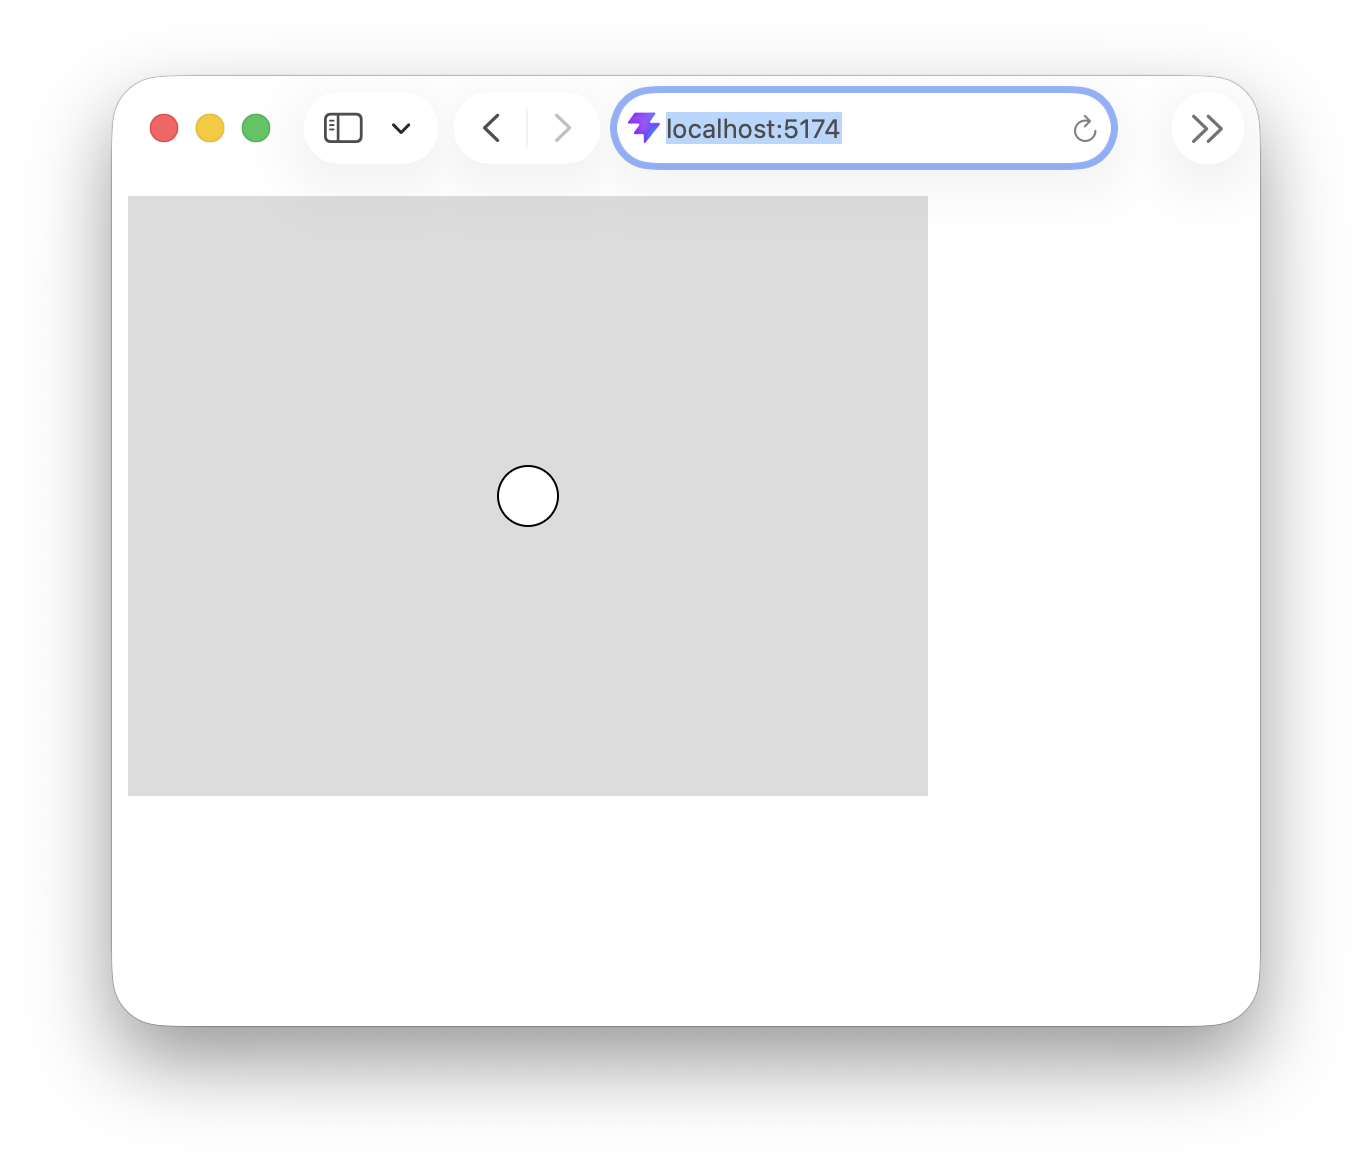
\includegraphics[width=0.5\textwidth]{figures/chapter01/browser-first-sketch.png}
    \caption{最初のスケッチの表示例}
    \label{fig:chapter01-first-sketch}
\end{figure}

5行目の\texttt{sketch}関数の引数名は、必ずしも\texttt{p}である必要はありません。
7行目や11行目で使っている\texttt{p.setup}や\texttt{p.draw}の\texttt{p}も、引数名を変えた場合は同じ名前にそろえます。
たとえば、引数名を\texttt{myP5}にした場合は、\texttt{myP5.createCanvas(...)}や\texttt{myP5.circle(...)}のように書きます（Listing~\ref{lst:chapter01-first-sketch-myP5}）。
慣習的に\texttt{p}という名前を使うのが慣習のようですので、この資料では\texttt{p}を使うことにします。

\begin{listing}[htbp]
\inputminted{ts}{listings/chapter01/first-sketch-myP5.ts}
\caption{最初のp5.jsスケッチの\texttt{p}を\texttt{myP5}に変更した例}
\label{lst:chapter01-first-sketch-myP5}
\end{listing}

\section{プログラムを書き換えてみよう}

プログラムが動いたら、少しだけ書き換えてみます。最初は、円の大きさ、円の位置、背景の色を変えるだけで十分です。この教材プロジェクトで最初に編集するファイルは、\texttt{typescript-p5/src/main.ts}です。
VS Codeのエクスプローラーで\texttt{typescript-p5}、\texttt{src}の順に開き、\texttt{main.ts}を選びます。そこで少しだけ数値を変えてみましょう。

たとえば、\texttt{p.circle(200, 150, 80)}の最後の数値を\texttt{120}に変えると、円が大きくなります。また、\texttt{p.background(240)}の数値を変えると、背景の明るさが変わります。

\begin{listing}[htbp]
\begin{minted}{ts}
p.background(220);
p.circle(200, 150, 120);
\end{minted}
\caption{背景と円の大きさを変更する例}
\label{lst:chapter01-edit-circle}
\end{listing}

別の章のサンプルを試すときは、VS Codeのエクスプローラーで\texttt{listings/}にある対象ファイルを開きます。開いた内容をすべて選んでコピーし、\texttt{typescript-p5/src/main.ts}を開いて内容をすべて選んで貼り付け、保存します。これにより\texttt{src/main.ts}の内容は上書きされます。

PowerShellを使う場合は、\texttt{typescript-p5/}を開いているターミナルで次のコマンドを実行します。

\begin{listing}[htbp]
\begin{minted}{powershell}
Copy-Item ..\listings\chapter02\points-and-lines.ts .\src\main.ts
\end{minted}
\caption{第2章のサンプルで\texttt{main.ts}を上書きするコマンド}
\label{lst:chapter01-copy-sample}
\end{listing}

\texttt{listings/}にあるファイルそのものは実行されません。コピーした\texttt{src/main.ts}が実行されます。保存またはコピーの後は、通常はViteを再起動しなくてもブラウザの表示が更新されます。画像、JSON、音を使うサンプルでは、それぞれの章で説明する素材ファイルも必要です。

書き換えたあとに期待どおりに動かないときは、まずVS Codeの赤い波線を確認します。次にターミナルの表示を確認し、最後にブラウザの表示を確認します。

\section{Gitで保存してみよう}

Gitでは、ファイルの変更を記録として保存できます。この記録をコミットと呼びます。コミットを作っておくと、あとで「どの時点で何を変更したか」を確認できます。この節では、開発サーバ用とは別にターミナルを開き、教材リポジトリのルートフォルダでGitコマンドを実行します。

まず、現在の変更状態を確認します。

\begin{listing}[htbp]
\begin{minted}{powershell}
git status
\end{minted}
\caption{Gitで変更状態を確認するコマンド}
\label{lst:chapter01-git-status}
\end{listing}

変更したファイルが表示されたら、次のように保存対象へ追加します。

\begin{listing}[htbp]
\begin{minted}{powershell}
git add typescript-p5/src/main.ts
\end{minted}
\caption{変更したファイルを保存対象へ追加するコマンド}
\label{lst:chapter01-git-add}
\end{listing}

この節ではGitコマンドを教材リポジトリのルートフォルダで実行します。一方、\texttt{npm}のコマンドは\texttt{typescript-p5/}で実行します。コマンドごとに実行する場所を確認しましょう。

最後に、変更内容を説明する短いメッセージを付けてコミットします。

\begin{listing}[htbp]
\begin{minted}{powershell}
git commit -m "最初のスケッチを変更"
\end{minted}
\caption{Gitで変更を保存するコマンド}
\label{lst:chapter01-git-commit}
\end{listing}

\begin{notebox}{コミットメッセージ}
コミットメッセージは、あとで見返したときに変更内容が分かるように書きます。最初は短い日本語で構いません。
\end{notebox}

\section{よくある間違い}

環境構築では、プログラムの文法とは別のところでつまずくことがあります。エラーが出たときは、あわてずに表示されたメッセージと作業しているフォルダを確認しましょう。

\begin{mistakebox}{コマンドを実行する場所が違う}
\texttt{npm install}や\texttt{npm run dev}は、教材プロジェクトのフォルダで実行します。\texttt{package.json}があるフォルダをVS Codeで開いているか確認してください。
\end{mistakebox}

\begin{mistakebox}{開発サーバを止めてしまう}
\texttt{npm run dev}を実行しているターミナルを閉じると、開発サーバも止まります。
作業中はそのターミナルを開いたままにしておきます。
止めたいときは、ターミナルで\texttt{Ctrl + C}を押します。
\end{mistakebox}

\begin{mistakebox}{Gitの保存とファイル保存を混同する}
VS Codeでファイルを保存することと、Gitでコミットすることは別の操作です。ファイル保存は現在の内容をディスクに書き込む操作で、コミットは変更の記録を作る操作です。
\end{mistakebox}

\section{まとめ}

この章では、Windows環境でTypeScript + p5.jsの教材を動かす準備をしました。VS Code、Git、Node.jsをインストールし、GitHubから教材を取得し、\texttt{npm install}と\texttt{npm run dev}でプログラムを実行しました。

また、最初のスケッチを少し書き換え、Gitで変更を保存する流れも確認しました。次章からは、p5.jsを使って図形を描く方法を少しずつ学んでいきます。

\section{演習問題}

この章の演習では、環境構築と最初の実行を確認します。すべてを暗記する必要はありません。コマンドを見ながら、同じ操作を自分のPCで再現できることを目指しましょう。

\begin{enumerate}
    \item VS Codeを起動し、教材フォルダを開いてください。
    \item VS Codeで新しいターミナルを開き、現在のフォルダが教材フォルダであることを確認してください。
    \item \texttt{node -v}と\texttt{npm -v}を実行し、バージョン番号が表示されることを確認してください。
    \item \texttt{npm install}を実行し、必要なライブラリをインストールしてください。
    \item \texttt{npm run dev}を実行し、ブラウザで教材ページを開いてください。
    \item 最初のスケッチで、円の大きさを変更してください。
    \item 最初のスケッチで、背景の明るさを変更してください。
    \item \texttt{git status}を実行し、変更されたファイルを確認してください。
    \item 変更したファイルを\texttt{git add}で追加し、\texttt{git commit}で保存してください。
    \item 挑戦問題として、円の位置、大きさ、背景色をすべて変更し、自分なりの最初の画面を作ってください。
\end{enumerate}
